\chapter{Grundlagen}\label{ch:grundlagen}

In diesem Kapitel sollen zunächst wichtige theoretische Grundlagen erklärt werden, die zum Verständnis der in den nachfolgenden Kapiteln beschriebenen Projektbearbeitungsschritte und -entscheidungen notwendig sind.

\section{Swift und SwiftUI}

Eine Festlegung, die bereits vor der Reimplementation der Apps getroffen wurde, ist die Wahl von Swift als Hauptprogrammiersprache der zu erstellenden iOS App. Die Programmiersprache wurde 2014 von Apple veröffentlicht und ersetzt seitdem Objective-C als die von Apple empfohlene Objektorientierte Sprache zur Erstellung von Applikationen für das Apple-Ökosystem mit den Betriebssystemderivaten Mac OS, iOS und bspw. auch Watch OS (Apple Watch). In der aktuellen Version 5 setzt Swift vielseitig etablierte Konzepte aus modernen Programmiersprachen um und ist hierbei nach dem subjektiven Empfinden des Projektteams leicht verständlich, schnell zu erlernen, sowie sehr kompakt. Zusammen mit Swift 5 wurde SwiftUI als deklaratives UI-Framework 2019 veröffentlicht, ergänzend zum herkömmlichen Constraint-basierten Layouting über UIView(Controller) und XIB/Storyboard-Dateien. SwiftUI orientiert sich an Frameworks wie React, bei denen Ansichten im Code definiert werden können, wodurch die Erstellung und Modifikation von Ansichten direkt im Editor geschehen kann, ohne die Notwendigkeit von etwaiger Controller-Logik, die UI-Elemente mit Code-Elementen (z.B. über die Annotation \texttt{@IBAction}) verbindet. Dies vereinfacht den Implementationsprozess, bringt jedoch auch verschiedene neue Architektur- und Datenflusskonzepte mit sich, die zunächst verstanden werden müssen, um SwiftUI effektiv und zielorientiert nutzen zu können.

\section{Datenfluss- und Architekturpatterns in SwiftUI}

In der nachfolgenden Sektion sollen zunächst die wesentlichsten Grundlagen des Datenflusses in SwiftUI-Ansichten erläutert werden. Anschließend werden verschiedene Patterns vorgestellt, die sich im Implementationskonzept wiederspiegeln und auch zukünftig idealerweise weiter genutzt werden sollten.

\subsection{Darstellung von View-Daten}

Im Unterschied zum imparativen UI-Programmierkonzept, bei dem konkrete Elemente der Ansicht, wie bspw. Labels oder Textfelder imparativ konfiguriert und mit den darzustellenden Daten ausgestattet werden, referenziert eine SwiftUI Ansicht (\enquote{View}) die darzustellenden Daten direkt aus dem Code, da sie selbst deklarativ in Form von Code geschrieben werden kann.

\begin{figure}[H]
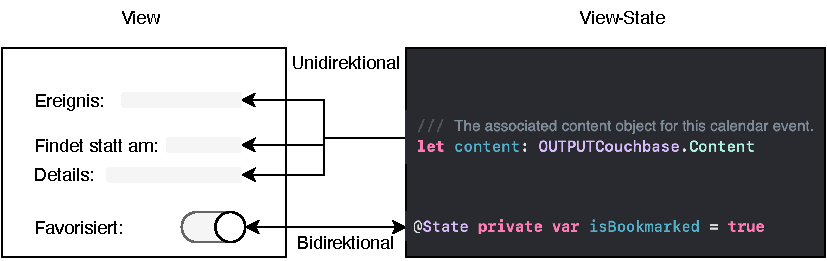
\includegraphics[width=\linewidth, bb=0 0 396 125]{swiftui.pdf}
\caption{Zwei wesentliche Arten des Datenflusses zwischen View und den in der View dargestellten Daten: unidirektional vs. bidirektional.}\label{fig:swiftui}
\end{figure}

\Cref{fig:swiftui} zeigt die zwei wesentlichsten Varianten, mithilfe derer Daten in der Ansicht dargestellt werden können: \textbf{unidirektional} und \textbf{bidirektional}. Bei der unidirektionalen Darstellung der Daten werden bei der Initialisierung der View die Daten im Konstruktor der View mitgegeben - da SwiftUI Views so genannte Structs sind, können die Daten im Verlauf der Zeit nicht mehr ändern (Struct-Felder sind \enquote{immutable}). SwiftUI rendert die assoziierten Elemente der View einmalig und verwendet diese nachfolgend zur Darstellung. Für viele Anwendungsfälle, in \Cref{fig:swiftui} anhang eines \enquote{Favorisieren-Buttons} illustriert, ist es jedoch notwendig, dass durch die View die dahinter liegenden Daten modifiziert werden. Hierfür wird der Property Wrapper \texttt{@State} bereitgestellt. Attribute, die hiermit ausgestattet werden, können während der Präsentation der View verändert werden. Eine Besonderheit hierbei ist, dass SwiftUI genau observiert, welche UI-Elemente durch das annotierte Attribut modifiziert oder konfiguriert werden, um bei einer Änderung des Attributs die entsprechenden Elemente neu zu rendern. Wird ein Datenattribut an eine Unteransicht weitergegeben, welche bspw. eine Detailansicht zu einem Objekt darstellt, dann wird das Attribut in der Unteransicht als \texttt{@Binding} referenziert.

\subsection{Coordinator-Pattern}

Um die Geschäftslogik der Anwendung von der Darstellungslogik weitestgehend zu separieren, kann das Coordinator-Pattern genutzt werden. Hierbei instanziiert die View ein eigenes Objekt, welches sie durch die \texttt{@StateObject} Annotation besitzt und kontrollieren kann, bspw. durch die Interaktion des Nutzers oder beim Erscheinen der Ansicht. Das Coordinator-Objekt macht die darzustellenden Datenattribute über die \texttt{@Published} Annotation nach außen verfügbar - so dass die View diese Datenattribute (ähnlich zu \texttt{@State} Datenattributen) verwenden und auf deren Änderungen reagieren kann.

\begin{figure}[H]
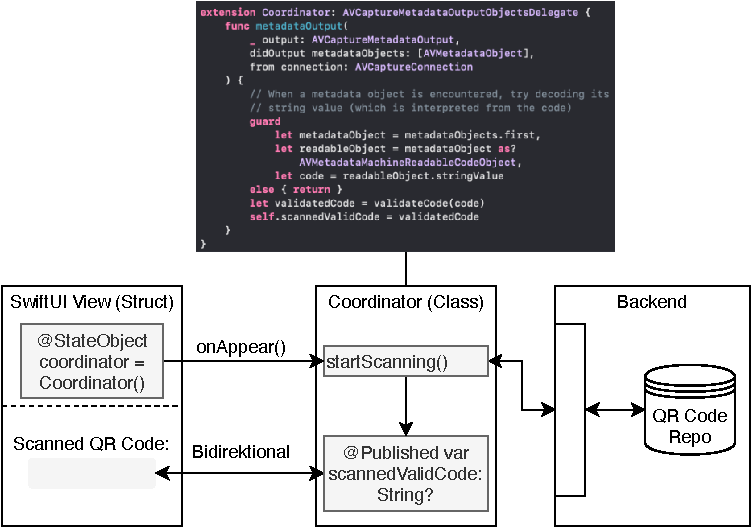
\includegraphics[width=\linewidth, bb=0 0 360 253]{coordinator.pdf}
\caption{Das Coordinator Pattern illustriert am Beispiel eines hypothetischen QR Code Scanners: Der Coordinator realisiert die Initialisierung des Scanners und die Validierung des Codes. Die View stellt den Code lediglich dar, sobald er gescannt wurde.}\label{fig:coordinator}
\end{figure}

In \Cref{fig:coordinator} ist das Pattern am Beispiel illustriert. Auch zu sehen ist hierbei, dass der Coordinator eine Klasse ist. Dies ist nützlich wenn bestimmte Protokolle (Swift-Interfaces) implementiert werden müssen, in diesem Beispiel \texttt{AVCaptureMetadataOutputObjectsDelegate} zur Reaktion auf gescannte QR Codes. In diesem Beispiel kann die View dieses Protokoll nicht implementieren, da das Protokoll implizit die Implementation durch eine Klasse erfordert.

\subsection{Environment-Pattern}

Als weiteres wichtiges Datenfluss-Pattern dient das Environment-Pattern. Hierbei wird, ähnlich zum Coordinator-Pattern, ein koordinierendes Umgebungsobjekt instanziiert und in der Besitz ergreifenden View als \texttt{@StateObject} markiert. Anschließend wird das Umgebungsobjekt im Environment der Unteransichten mitgegeben, über den ViewModifier \texttt{view.environmentObject(object)}. Dies ist zum Beispiel sinnvoll, wenn eine Unteransicht bestimmte Daten aus dem Kontext beziehen und/oder modifizieren möchte.

\begin{figure}[H]
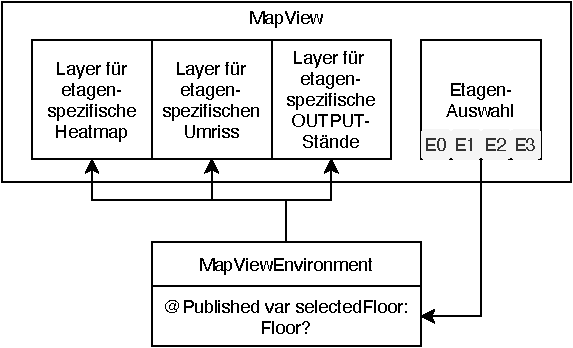
\includegraphics[width=\linewidth, bb=0 0 275 167]{environment.pdf}
\caption{Das Environment Pattern illustriert am Beispiel der Map View: Die Map View erstellt ihr eigenes Environment und gibt dieses an ihre Unteransichten weiter. Somit kann die gewählte Etage von einer Unteransicht modifiziert werden, von anderen Unteransichten wird sie lediglich dargestellt.}\label{fig:coordinator}
\end{figure}

In \Cref{fig:coordinator} ist dieses Pattern am Beispiel illustriert. Ein großer Vorteil des Patterns ist, dass das über den ViewModifier weitergegebene Umgebungsobjekt transitiv an alle weiteren Unteransichten weitergeleitet wird, die sich möglicherweise in dieser Unteransicht befinden. Der Bezug des Objektes findet anschließend über \texttt{@EnvironmentObject var object} statt. Ein Problem hierbei ist, dass das Objekt nicht optional weitergegeben werden kann, was die Preview der SwiftUI Unteransichten erschwert. Die hierfür applizierte Lösung hierfür wird später im Konzeptkapitel näher beschrieben.

\subsection{View-Proxy-Pattern}

Die Grundlagen des Environment-Pattern und des Coordinator-Pattern können weiterhin genutzt werden, um bestimmte Bestandteile der Geschäftslogik im View-Proxy-Pattern zu separieren. Hierbei wird eine dedizierte View erstellt, deren Aufgabe es ist, bestimmte Datenverarbeitungsoperationen durchzuführen und bei Beendigung dessen die Produkte dieser Operation als Umgebungsobjekt bzw. Proxy-Objekt der inneren View bereitzustellen. Hierfür wird die innere View der Proxy View als \texttt{@ViewBuilder}-Closure übergeben. Ein klassisches Beispiel für das View-Proxy-Pattern ist der von SwiftUI standardmäßig bereitgestellte \texttt{GeometryReader}, welcher als View genutzt werden kann, um ein Proxy-Objekt für die Geometrie der View zu erstellen, bspw. um die Größe einer Ansicht zu bestimmen. Im Konzept der App wird dies später für die Initialisierung der Datenbank und Replikatoren adaptiert und an dieser Stelle noch einmal genauer beschrieben.

\subsection{Eventbasierte Datenflüsse}

Eventbasierte Datenflüsse stellen ein weiteres wichtiges Pattern für die Weitergabe von Daten dar. Bei den bisherigen Pattern wurden lediglich Methoden vorgestellt, mithilfe derer sich ein Datenfluss zwischen mehreren Views in \textit{derselben} View-Hierarchie realisieren lässt. In manchen Fällen ist es jedoch notwendig, dass bestimmte Datenverarbeitungsprozesse von der View-Hierarchie entkoppelt werden, beispielsweise bei periodischen Hintergrundprozessen. Um in diesem Fall dennoch bspw. eine entsprechende Meldung im UI anzuzeigen, können globale Events ausgelöst werden, die von Observern innerhalb der View aufgegriffen und zur Anzeige verarbeitet werden können. Hierbei kann das \texttt{NotificationCenter} genutzt werden, um Nachrichten auf einen Event-Bus zu pushen und innerhalb der View über einen so genannten \texttt{Publisher} zu empfangen. Auch dieses Pattern wird später noch an einem konkreten Beispiel im Rahmen des Implementationskonzeptes zu den Spiel-Errungenschaften gezeigt.
